\documentclass[10pt,a4paper]{article}
\usepackage[margin=1.7cm,top=1.8cm,bottom=1.8cm]{geometry}
\usepackage[T1]{fontenc}
\usepackage[utf8]{inputenc}
\usepackage{lmodern,microtype}
\usepackage{xcolor}
\usepackage{booktabs,tabularx,array}
\usepackage{amsmath,amssymb}
\usepackage{enumitem}
\usepackage{tikz}
\usetikzlibrary{arrows.meta,positioning,calc,fit,shapes.geometric,backgrounds}
\usepackage{hyperref}

% Project Color Palette
\definecolor{navy}{HTML}{123047}
\definecolor{teal}{HTML}{007C7A}
\definecolor{sky}{HTML}{DCEFF1}
\definecolor{orange}{HTML}{E67E22}
\definecolor{pale}{HTML}{F4F6F7}

\hypersetup{
  colorlinks=true,
  linkcolor=navy,
  citecolor=navy,
  urlcolor=navy,
  pdftitle={Semi-Humanoid Robotic Platform -- Project Overview}
}

\setlength{\parindent}{0pt}
\setlength{\parskip}{0.32em}
\renewcommand{\arraystretch}{1.12}
\newcolumntype{Y}{>{\raggedright\arraybackslash}X}

\begin{document}

% Header Block
\begin{center}
  {\Large\bfseries A Modular General-Purpose Semi-Humanoid Robotic Platform\par}
  \vspace{0.25em}
  {\large\color{navy}\textbf{Technical Project Overview and Conceptual Mechatronic Architecture}\par}
  \vspace{0.35em}
  {\footnotesize\textbf{Graduation Project Technical Overview} \quad|\quad Faculty of Engineering, Ain Shams University \quad|\quad September 2026\par}
  \vspace{0.25em}
  \hrule height 1pt
\end{center}
\vspace{-0.5em}

\begin{abstract}
\footnotesize
This report presents the conceptual design, systems engineering architecture, and technical specification for an 18-Degree-of-Freedom (DoF) modular semi-humanoid robotic platform. Grounded in the VDI~2206 mechatronic systems design methodology, the platform addresses the trilemma between single-purpose automated machinery and cost-prohibitive bipedal humanoids. The robot integrates a high-traction differential-drive wheeled base, a fixed ergonomic space-frame torso, dual 6-DoF anthropomorphic arms featuring a hybrid Quasi-Direct Drive (QDD) and serial bus servo actuation topology, symmetrical parallel-jaw grippers, an active 2-DoF RGB-D perception head, and an isolated 24V $\text{LiFePO}_4$ power infrastructure. To decouple physical execution from cognitive intent, the system formalizes a sandboxed \emph{Task Port} and a 4-tier multi-rate software hierarchy ($5\text{ Hz}$ AI cognition to $1\text{ kHz}$ hard real-time motor commutation). Validated against standardized RoboCup@Home benchmarks, the core platform achieves an operational reach of $500\text{--}1350\text{ mm}$, an all-up mass $\le 55\text{ kg}$, and an itemized build budget of 432,915 EGP ($\sim$\$8,900 USD).
\end{abstract}
\vspace{-0.3em}

\noindent{\footnotesize\textbf{Keywords:} Semi-Humanoid Robot; VDI 2206 Mechatronics; Task Port; Hybrid QDD Actuation; Multi-Rate Architecture.}

% -----------------------------------------------------------------------------
% SECTION 1: INTRODUCTION & METHODOLOGY
% -----------------------------------------------------------------------------
\vspace{-0.4em}
\section{Executive Context, Motivation, and Design Philosophy}
\label{sec:intro}
\vspace{-0.2em}
\textbf{The Service Robotics Trilemma:} Service, domestic, and laboratory automation currently faces a sharp technological divide. Rigid single-purpose robotic workcells lack task adaptability, while full-scale bipedal humanoids incur prohibitive capital costs ($>\$100\text{k}\text{--}\$250\text{k}$), severe balance instabilities, and non-negligible idle energy consumption. As established in contemporary Cyber-Physical Systems (CPS) literature for Industry 5.0, a wheeled \emph{semi-humanoid} mobile manipulator resolves this trilemma: a differential-drive base ensures unconditional static overturning stability, while an anthropomorphic upper body provides manipulation dexterity in human-designed spaces.

\textbf{Core Architectural Principle -- Capability vs. Intent:} Traditional mobile robots hardcode task-specific behaviors into low-level control loops. In this project, we enforce a strict separation of concerns:
\begin{quote}
\centering\footnotesize\itshape
``The platform provides deterministic physical capability; the application layer provides cognitive intent.''
\end{quote}
The physical body exposes a fixed, stable set of verified motion and perception primitives via a sandboxed \textbf{Task Port}. Downstream users, task-level Behavior Trees, or foundation Vision-Language-Action (VLA) models interact exclusively through standardized ROS~2 Action interfaces, preventing algorithmic software failures from compromising hardware safety.

\textbf{VDI 2206 Mechatronic Methodology:} System development strictly follows the VDI~2206 guideline~\cite{vdi2206}. The macro V-model guides progression from empirical task analysis to cross-domain conceptual design, followed by concurrent mechanical, electrical, and software engineering, ascending through Software-in-the-Loop (SIL), Hardware-in-the-Loop (HIL), and physical verification. Micro-cycles of problem-solving (\emph{Situation Analysis $\to$ Target Formulation $\to$ Synthesis $\to$ Analysis/Evaluation $\to$ Decision $\to$ Planning}) prevent premature hardware locking. 

In machine dynamics, joint stiffness $K$ and distal moving mass $M$ govern the mechanical natural frequency $\omega_n = \sqrt{K/M}$ and closed-loop settling time $t_{\text{settling}} \approx 4 / (\zeta \omega_n)$. Minimizing distal link inertia by concentrating mass proximally raises structural resonance, suppresses vibrations, and enables high-gain, compliant manipulation.

% -----------------------------------------------------------------------------
% SECTION 2: EMPIRICAL TASKS & REQUIREMENTS SPECIFICATION
% -----------------------------------------------------------------------------
\vspace{-0.4em}
\section{Empirical Task Formulation, Benchmarks, and Requirements}
\label{sec:tasks_reqs}
\vspace{-0.2em}
\textbf{Empirical Benchmarks:} Rather than designing around an arbitrary task, physical boundaries are derived from international service robotics standards (RoboCup@Home~\cite{robocupathome}, World Robot Summit, and ISO~13482:2014 safety standards~\cite{iso13482}):
\begin{itemize}[leftmargin=1.2em,noitemsep,topsep=1pt]
  \item \emph{Doorway \& Aisle Clearance:} Standard interior apertures ($750\text{--}900\text{ mm}$) dictate base width $\le 550\text{ mm}$ for collision-free passage.
  \item \emph{Working Height Envelopes:} Standard dining tables ($750\text{ mm}$), kitchen counters ($900\text{ mm}$), and mid-level shelving ($1200\text{ mm}$) establish a continuous required vertical reach band of $500\text{--}1350\text{ mm}$ above floor level.
  \item \emph{Everyday Workpiece Masses:} Domestic tableware, beverage containers, and packaged items ($0.1\text{--}1.0\text{ kg}$) require $\ge 1.0\text{ kg}$ nominal continuous payload capacity at full horizontal arm extension ($625\text{ mm}$).
\end{itemize}

\textbf{Platform Validation Tasks:} The integrated platform is validated against two canonical reference benchmarks:
\begin{enumerate}[leftmargin=1.2em,noitemsep,topsep=1pt]
  \item \emph{Primary Benchmark (Autonomous Voice Pick-and-Place):} Speech input parsed by Whisper STT~\cite{whisper}; intent resolved by an OpenVLA~\cite{openvla} planner into typed Task Port actions; differential base navigates to table via Nav2~\cite{nav2}; RealSense head estimates 6D object pose; MoveIt~2~\cite{moveit2} executes collision-free grasp; base transits and deposits item onto target surface.
  \item \emph{Secondary Benchmark (Web Dashboard Teleoperation \& Task Programming):} Operator jogs base and arms via low-latency WebRTC browser joysticks, monitors real-time telemetry/alarms, and records waypoint macros for autonomous trajectory replay.
\end{enumerate}

\textbf{Engineering Requirements Specification (\emph{Anforderungsliste}):} Following VDI~2206, Table~\ref{tab:reqs_summary} compiles the foundational engineering requirements, classified into Fixed Requirements (FF / Demand) and Range Requirements (BF / Wish), quantitative (\emph{quan}) and qualitative (\emph{qual}).

\begin{table}[ht]
\vspace{-0.2em}
\centering\scriptsize
\caption{Consolidated VDI 2206 Engineering Requirements Specification (\emph{Anforderungsliste}).}
\label{tab:reqs_summary}
\vspace{-0.3em}
\begin{tabularx}{\textwidth}{@{}llXllY@{}}
\toprule
\textbf{ID} & \textbf{Category} & \textbf{Parameter Metric} & \textbf{Target Value} & \textbf{Type} & \textbf{Verification Method} \\
\midrule
G01 & Geometry & Footprint envelope diameter & $\le 550\text{ mm}$ (Length $\le 600\text{ mm}$) & BF / quan & CAD audit \& physical passage test \\
G02 & Geometry & Doorway aperture passage & Clearance margin $\ge 100\text{ mm}$ in $750\text{ mm}$ doors & FF / quan & Physical benchmark doorway trial \\
G03 & Geometry & Platform height \& total mass & Height: $1200\text{--}1300\text{ mm}$; Wet mass $\le 55\text{ kg}$ & BF / quan & Coordinate gauge \& calibrated scale \\
K01 & Kinematics & Active Degrees of Freedom (DoF) & \textbf{18 Active DoF} (Base: 2, Arms: 12, Grippers: 2, Head: 2) & FF / quan & Topological kinematic joint audit \\
K02 & Kinematics & Base drivetrain topology & Coaxial differential drive + dual swivel casters & FF / qual & Trajectory tracking \& pivot-spin trial \\
K03 & Kinematics & Vertical manipulation envelope & $500\text{ mm}$ (table-low) to $\ge 1350\text{ mm}$ (high shelf) & FF / quan & TCP reach calibration across workspace \\
K04 & Kinematics & Horizontal dual-arm bimanual span & Symmetric span $\ge 1200\text{ mm}$; single arm reach $\ge 625\text{ mm}$ & BF / quan & Forward kinematic envelope mapping \\
D01 & Dynamics & Arm payload capacity at full reach & Nominal: $\ge 1.0\text{ kg}$; Peak static holding: $\ge 1.5\text{ kg}$ & FF / quan & Static holding test at full horizontal reach \\
D02 & Dynamics & Parallel gripper stroke \& clamping & Stroke: $0\text{--}85\text{ mm}$; Clamping force: $15\text{--}35\text{ N}$ & FF / quan & Calibrated load-cell grip trial \\
D03 & Dynamics & Base transit speed & $0.6\text{--}0.8\text{ m/s}$ (ISO 13482 indoor safety limit) & BF / quan & Laser-timed linear velocity profile \\
D04 & Dynamics & Cartesian repeatability & $\le \pm 2.0\text{ mm}$ under full payload & BF / quan & Dial indicator multi-cycle test \\
D05 & Dynamics & Structural settling time & $t_{\text{settling}} \le 0.5\text{ s}$ after rapid slew ($\zeta \ge 0.6$) & BF / quan & Accelerometer vibration decay probe \\
E01 & Electrical & Primary DC power bus & $24.0\text{ V}$ nominal ($8\text{S LiFePO}_4$ battery pack) & FF / quan & Oscilloscope rail voltage logging \\
E02 & Electrical & Operational battery runtime & $\ge 3.0\text{ h}$ continuous mixed cycle ($\ge 5.0\text{ h}$ idle) & BF / quan & Automated execution loop to low-SoC \\
E03 & Electrical & Hardware E-Stop isolation & Actuator power disconnected in $\le 10\text{ ms}$ & FF / quan & Oscilloscope timing of contactor drop \\
C01 & Control & Joint control cycle frequency & $\ge 500\text{ Hz}$ (Target: $1000\text{ Hz}$) on native MCU & FF / quan & FreeRTOS task jitter telemetry \\
C02 & Control & Subsystem communication fieldbus & CAN 2.0B / TWAI ($\ge 1\text{ Mbps}$) \& half-duplex TTL & FF / qual & Protocol analyzer packet loss check \\
C03 & Control & Device-level modular abstraction & Each assembly operates as an independent node & FF / qual & Hot-unplug diagnostic isolation audit \\
S01 & Sensing & Base obstacle detection coverage & $360^\circ$ planar LiDAR + ultrasonic blind-spot ring & FF / quan & Blind-spot mapping with standard targets \\
S02 & Sensing & Active visual perception & Active stereo RGB-D camera on 2-DoF gimbal & FF / qual & Point cloud density \& registration audit \\
A01 & Software & Middleware framework & ROS~2 LTS (Humble/Jazzy)~\cite{ros2} with PREEMPT\_RT & FF / qual & DDS QoS latency \& jitter audit \\
A02 & Software & Task Port abstraction interface & Sandboxed Action Servers (`/navigate`, `/pick`, `/place`) & FF / qual & End-to-end task script invocation \\
H01 & HMI & Web-based operational dashboard & React/WebRTC dashboard with teleop latency $\le 80\text{ ms}$ & FF / quan & Network packet round-trip time probe \\
H02 & HMI & Physical torso maintenance panel & OLED status display, RJ-45 GbE \& dual USB 3.0 ports & FF / qual & Functional inspection of bulkhead panel \\
SF1 & Safety & Human-co-presence safety & Dynamic speed scaling \& force veto per ISO 13482 & FF / qual & Contact stop \& obstacle detection tests \\
\bottomrule
\end{tabularx}
\vspace{-0.5em}
\end{table}

\textbf{Rationale for Core Architectural Decisions:}
\begin{enumerate}[leftmargin=1.2em,noitemsep,topsep=1pt]
  \item \emph{Differential vs. Mecanum Drive:} Mecanum wheels exhibit $15\text{--}25\%$ transverse dead-reckoning slip on smooth/carpeted floors, induce severe high-frequency roller vibrations that degrade camera point clouds, and waste battery power. Differential drive provides high traction, simple odometry, zero-radius pivot spinning, and rugged reliability.
  \item \emph{Dual 6-DoF Arms over 7-DoF:} 6-DoF arms fully span $SE(3)$ task space. Omitting a redundant 7th joint eliminates $1.5\text{--}2.0\text{ kg}$ of cantilever mass per arm, raising the joint natural frequency $\omega_n$, reducing settling time, eliminating kinematic singularity search latency, and halving control bus packet overhead.
  \item \emph{Fixed Torso over Telescopic Column:} Motorized vertical lift columns add $>12\text{ kg}$ of dead mass, elevate the center of gravity, and suffer mechanical guide binding under bimanual cantilever loads. A fixed structural mast (shoulder axis at $950\text{ mm}$) spans $500\text{--}1350\text{ mm}$ reach, covering tables, counters, and eye-level shelves at zero mechanical risk.
  \item \emph{2-Finger Parallel Grippers over Multi-Finger Hands:} Underactuated multi-finger hands suffer frequent cable stretch and low pinch forces. Symmetrical parallel-jaw grippers with Shore-A 60 compliant silicone pads deliver deterministic force/form closure ($15\text{--}35\text{ N}$) and sensorless grasp verification via motor phase current monitoring.
\end{enumerate}

% -----------------------------------------------------------------------------
% SECTION 3: FUNCTIONAL STRUCTURE & SYSTEM ARCHITECTURE
% -----------------------------------------------------------------------------
\vspace{-0.4em}
\section{Functional Flow Modeling and System Mechatronic Architecture}
\label{sec:architecture}
\vspace{-0.2em}
\textbf{Functional Structure (VDI 2206):} The robot is modeled as a cybernetic system transforming three physical flows across its boundary $\mathcal{B}_{\text{system}}$: Material ($\mathbf{M}$), Energy ($\mathbf{E}$), and Information ($\mathbf{I}$), as illustrated in Fig.~\ref{fig:functional_structure}.

\begin{figure}[ht]
\vspace{-0.2em}
\centering
\resizebox{0.92\textwidth}{!}{%
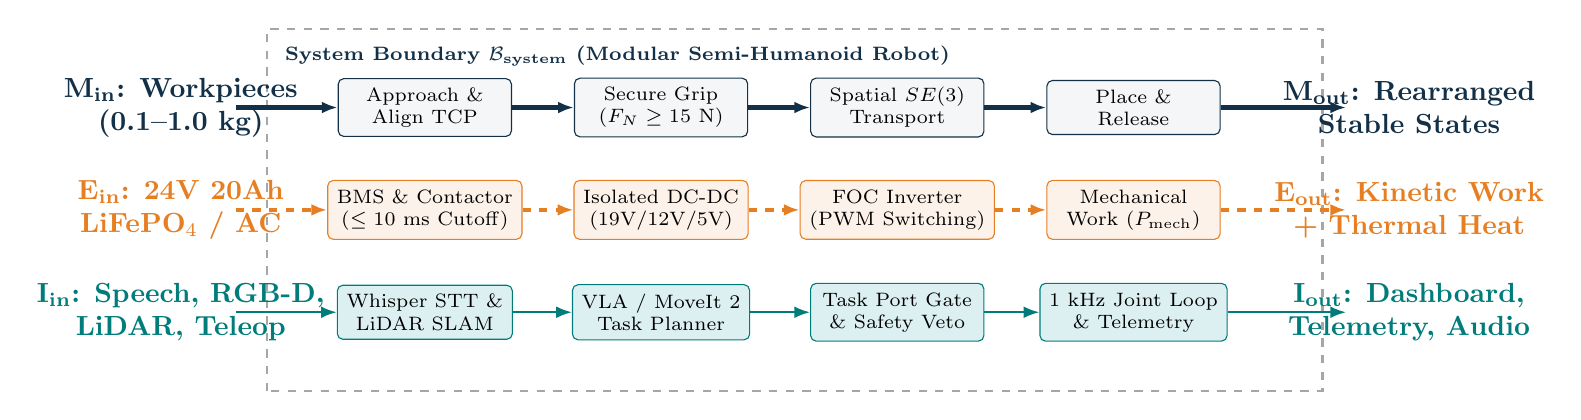
\begin{tikzpicture}[every node/.style={font=\scriptsize,align=center},box/.style={draw=navy,fill=white,rounded corners=2pt,minimum width=2.2cm,minimum height=0.6cm}]
  % Boundary
  \draw[dashed,thick,gray!70] (-1.2,-2.3) rectangle (12.2,2.3);
  \node[anchor=north west,font=\bfseries\scriptsize,navy] at (-1.1,2.2) {System Boundary $\mathcal{B}_{\text{system}}$ (Modular Semi-Humanoid Robot)};

  % Material Flow
  \node[font=\bfseries,navy] at (-2.3,1.3) {$\mathbf{M}_{\text{in}}$: Workpieces\\(0.1--1.0 kg)};
  \node[box,draw=navy,fill=pale] (m1) at (0.8,1.3) {Approach \&\\Align TCP};
  \node[box,draw=navy,fill=pale] (m2) at (3.8,1.3) {Secure Grip\\($F_N \ge 15\text{ N}$)};
  \node[box,draw=navy,fill=pale] (m3) at (6.8,1.3) {Spatial $SE(3)$\\Transport};
  \node[box,draw=navy,fill=pale] (m4) at (9.8,1.3) {Place \&\\Release};
  \node[font=\bfseries,navy] at (13.3,1.3) {$\mathbf{M}_{\text{out}}$: Rearranged\\Stable States};
  \draw[-{Latex[length=2mm]},line width=1.5pt,navy] (-1.6,1.3) -- (m1);
  \draw[-{Latex[length=2mm]},line width=1.5pt,navy] (m1) -- (m2);
  \draw[-{Latex[length=2mm]},line width=1.5pt,navy] (m2) -- (m3);
  \draw[-{Latex[length=2mm]},line width=1.5pt,navy] (m3) -- (m4);
  \draw[-{Latex[length=2mm]},line width=1.5pt,navy] (m4) -- (12.5,1.3);

  % Energy Flow
  \node[font=\bfseries,orange] at (-2.3,0.0) {$\mathbf{E}_{\text{in}}$: 24V 20Ah\\$\text{LiFePO}_4$ / AC};
  \node[box,draw=orange,fill=orange!10] (e1) at (0.8,0.0) {BMS \& Contactor\\($\le 10\text{ ms}$ Cutoff)};
  \node[box,draw=orange,fill=orange!10] (e2) at (3.8,0.0) {Isolated DC-DC\\(19V/12V/5V)};
  \node[box,draw=orange,fill=orange!10] (e3) at (6.8,0.0) {FOC Inverter\\(PWM Switching)};
  \node[box,draw=orange,fill=orange!10] (e4) at (9.8,0.0) {Mechanical\\Work ($P_{\text{mech}}$)};
  \node[font=\bfseries,orange] at (13.3,0.0) {$\mathbf{E}_{\text{out}}$: Kinetic Work\\+ Thermal Heat};
  \draw[-{Latex[length=2mm]},line width=1.2pt,dashed,orange] (-1.6,0.0) -- (e1);
  \draw[-{Latex[length=2mm]},line width=1.2pt,dashed,orange] (e1) -- (e2);
  \draw[-{Latex[length=2mm]},line width=1.2pt,dashed,orange] (e2) -- (e3);
  \draw[-{Latex[length=2mm]},line width=1.2pt,dashed,orange] (e3) -- (e4);
  \draw[-{Latex[length=2mm]},line width=1.2pt,dashed,orange] (e4) -- (12.5,0.0);

  % Information Flow
  \node[font=\bfseries,teal] at (-2.3,-1.3) {$\mathbf{I}_{\text{in}}$: Speech, RGB-D,\\LiDAR, Teleop};
  \node[box,draw=teal,fill=sky] (i1) at (0.8,-1.3) {Whisper STT \&\\LiDAR SLAM};
  \node[box,draw=teal,fill=sky] (i2) at (3.8,-1.3) {VLA / MoveIt 2\\Task Planner};
  \node[box,draw=teal,fill=sky] (i3) at (6.8,-1.3) {Task Port Gate\\\& Safety Veto};
  \node[box,draw=teal,fill=sky] (i4) at (9.8,-1.3) {1 kHz Joint Loop\\\& Telemetry};
  \node[font=\bfseries,teal] at (13.3,-1.3) {$\mathbf{I}_{\text{out}}$: Dashboard,\\Telemetry, Audio};
  \draw[-{Latex[length=2mm]},thick,teal] (-1.6,-1.3) -- (i1);
  \draw[-{Latex[length=2mm]},thick,teal] (i1) -- (i2);
  \draw[-{Latex[length=2mm]},thick,teal] (i2) -- (i3);
  \draw[-{Latex[length=2mm]},thick,teal] (i3) -- (i4);
  \draw[-{Latex[length=2mm]},thick,teal] (i4) -- (12.5,-1.3);
\end{tikzpicture}%
}
\vspace{-0.6em}
\caption{Tripartite functional flow structure decomposition ($\mathbf{M}$, $\mathbf{E}$, $\mathbf{I}$) across the mechatronic system boundary.}
\label{fig:functional_structure}
\vspace{-0.4em}
\end{figure}

\textbf{Hierarchical Multi-Rate Execution Topology:} To maintain control stability, software tasks are partitioned across four explicit frequency domains:
\begin{itemize}[leftmargin=1.2em,noitemsep,topsep=1pt]
  \item \emph{Tier 1: Cognition \& HRI ($5\text{--}10\text{ Hz}$):} Whisper STT, OpenVLA action chunk proposal, WebRTC video streaming.
  \item \emph{Tier 2: Mission \& Planning ($30\text{--}50\text{ Hz}$):} BehaviorTree.CPP task sequencer, Nav2 local costmaps, MoveIt~2 Cartesian trajectory planning.
  \item \emph{Tier 3: Robot Integration \& Middleware ($100\text{--}250\text{ Hz}$):} `ros2\_control` resource management, cubic Hermite spline interpolation, Unscented Kalman Filter (UKF) state estimation.
  \item \emph{Tier 4: Safety \& Actuation ($500\text{--}1000\text{ Hz}$):} Native FreeRTOS loops on distributed ESP32 MCUs, 1 Mbps CAN bus cyclic commutation, actuator FOC current loops, thermal watchdogs, and hardware E-Stop monitoring.
\end{itemize}

% \textbf{Mathematical Command Contract \& Safety Veto:} Every AI proposal $\Delta\mathbf{x}_{\text{AI}}$ must be projected into an admissible constraint set:
% \begin{equation}
% \mathbf{x}_{\text{ref}} = \Pi_{\mathcal{F}(\mathbf{q},\mathcal{E},\mathcal{S})} \left( \mathbf{x} + \Delta\mathbf{x}_{\text{AI}} \right) = \arg\min_{\mathbf{y} \in \mathcal{F}} \frac{1}{2} \|\mathbf{y} - (\mathbf{x} + \Delta\mathbf{x}_{\text{AI}})\|^2_{\mathbf{W}}
% \end{equation}
% where $\mathcal{F} = \mathcal{C}_{\text{kin}} \cap \mathcal{C}_{\text{stab}} \cap \mathcal{C}_{\text{env}} \cap \mathcal{C}_{\text{safe}}$ enforces joint limits, Zero-Moment Point (ZMP) dynamic stability inside the wheel polygon, Signed Distance Field (SDF) self-collision bounds, and ISO~13482 human velocity clamping. Violations trigger an observable `SafetyProjectionVeto` recovery event, preventing silent runaway failures.

% -----------------------------------------------------------------------------
% SECTION 4: DETAILED SUBSYSTEM MECHATRONIC DESIGN
% -----------------------------------------------------------------------------
\vspace{-0.4em}
\section{Detailed Subsystem Engineering (The 8 Modular Devices)}
\label{sec:subsystems}
\vspace{-0.2em}
In accordance with the \emph{Device-Level} architecture, each subsystem is encapsulated as an independent node coordinated by an ESP32 microcontroller over CAN (TWAI) or USB/Ethernet to the primary NVIDIA Jetson Orin NX host.

\begin{figure}[ht]
\vspace{-0.3em}
\centering
\resizebox{0.94\textwidth}{!}{%
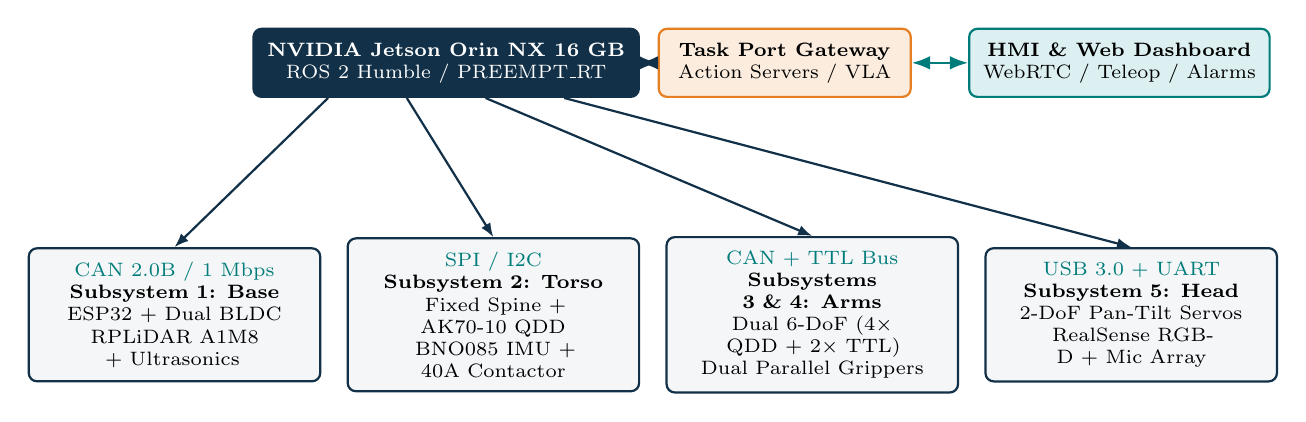
\begin{tikzpicture}[
  >=Latex,
  every node/.style={font=\scriptsize,align=center},
  hub/.style={draw=navy,fill=navy,text=white,rounded corners=3pt,thick,minimum height=0.82cm,inner sep=5pt},
  gateway/.style={draw=orange,fill=orange!15,rounded corners=3pt,thick,minimum height=0.82cm,inner sep=5pt},
  interface/.style={draw=teal,fill=sky,rounded corners=3pt,thick,minimum height=0.82cm,inner sep=5pt},
  device/.style={draw=navy,fill=pale,rounded corners=3pt,thick,text width=3.35cm,minimum width=3.62cm,minimum height=1.05cm,inner sep=5pt},
  link/.style={-{Latex[length=1.8mm]},thick,navy}
]
  % Compute, task interface, and operator interface form the upper tier.
  \node[hub,minimum width=4.0cm] (jetson) at (4.8,3.2) {\textbf{NVIDIA Jetson Orin NX 16 GB}\\ROS 2 Humble / PREEMPT\_RT};
  \node[gateway,minimum width=3.2cm] (taskport) at (9.1,3.2) {\textbf{Task Port Gateway}\\Action Servers / VLA};
  \node[interface,minimum width=3.35cm] (hmi) at (13.35,3.2) {\textbf{HMI \& Web Dashboard}\\WebRTC / Teleop / Alarms};
  \draw[thick,navy,<->] (jetson.east) -- (taskport.west);
  \draw[thick,teal,<->] (taskport.east) -- (hmi.west);

  % Device-level subsystem cards form a separate lower tier.
  \node[device] (base) at (1.35,0) {\textcolor{teal}{CAN 2.0B / 1 Mbps}\\\textbf{Subsystem 1: Base}\\ESP32 + Dual BLDC\\RPLiDAR A1M8 + Ultrasonics};
  \node[device] (torso) at (5.4,0) {\textcolor{teal}{SPI / I2C}\\\textbf{Subsystem 2: Torso}\\Fixed Spine + AK70-10 QDD\\BNO085 IMU + 40A Contactor};
  \node[device] (arms) at (9.45,0) {\textcolor{teal}{CAN + TTL Bus}\\\textbf{Subsystems 3 \& 4: Arms}\\Dual 6-DoF (4$\times$ QDD + 2$\times$ TTL)\\Dual Parallel Grippers};
  \node[device] (head) at (13.5,0) {\textcolor{teal}{USB 3.0 + UART}\\\textbf{Subsystem 5: Head}\\2-DoF Pan-Tilt Servos\\RealSense RGB-D + Mic Array};

  % Fan-out links stay separate and unlabeled; protocols are in each card.
  % Ordered source and destination points prevent the links from crossing.
  \begin{scope}[on background layer]
    \draw[link] ([xshift=-1.5cm]jetson.south) -- (base.north);
    \draw[link] ([xshift=-0.5cm]jetson.south) -- (torso.north);
    \draw[link] ([xshift=0.5cm]jetson.south) -- (arms.north);
    \draw[link] ([xshift=1.5cm]jetson.south) -- (head.north);
  \end{scope}
\end{tikzpicture}%
}
\vspace{-0.6em}
\caption{System mechatronic topology: Tier-1 real-time fieldbuses, central edge compute host, and Task Port gateway.}
\label{fig:mechatronic_topology}
\vspace{-0.3em}
\end{figure}

\textbf{1. Subsystem 1: Mobile Base Device:} Differential drive kinematics powered by $2\times$ 24V 100W BLDC gearmotors ($\sim 30:1$ planetary reduction, optical quadrature encoders) driving $200\text{ mm}$ vulcanized rubber wheels. Dual $100\text{ mm}$ swivel casters provide a stable 4-point footprint clearing $15\text{ mm}$ cable thresholds. Perception includes a Slamtec RPLiDAR A1M8 ($360^\circ$ planar scan, 12 m range) fused with $4\times$ HC-SR04 ultrasonic sensors for blind-zone detection. Controlled by an ESP32-WROOM-32 via a custom dual H-bridge carrier PCB.

\textbf{2. Subsystem 2: Fixed Torso \& Structural Mast:} A rigid 6061-T6 aluminum extrusion spine ($30\times 30\text{ mm}$ and $40\times 40\text{ mm}$) with shoulder yoke at $950\text{ mm}$. Incorporates a waist tilt joint powered by a CubeMars AK70-10 QDD actuator ($24.8\text{ N}\cdot\text{m}$ peak torque, 10:1 planetary reduction, 14-bit absolute encoder, integrated FOC driver) and a BNO085 9-DoF IMU. Houses the main power contactor, fuse blocks, and active compute cooling.

\textbf{3. Subsystems 3 \& 4: Dual 6-DoF Manipulator Arm Devices:} Anthropomorphic 6-DoF configuration ($SE(3)$ reach: $625\text{ mm}$) featuring an innovative hybrid actuation topology:
\begin{itemize}[leftmargin=1.2em,noitemsep,topsep=1pt]
  \item \emph{Proximal Joints (Shoulder Pitch/Roll/Yaw, Elbow Pitch):} $4\times$ CubeMars AK70-10 QDD actuators per arm, delivering low gear ratios ($10:1$), exceptional backdrivability, high impact resistance, and proprioceptive current-based torque sensing.
  \item \emph{Distal Wrist Joints (Wrist Pitch and Roll):} $2\times$ Feetech STS3215 serial bus servos ($12\text{V}$, $2.9\text{ N}\cdot\text{m}$ stall, half-duplex TTL UART @ 1 Mbps), reducing distal arm weight by $>90\%$ and actuator cost by $>75\%$.
\end{itemize}
Coordinated by a dedicated ESP32 per arm on a custom interface PCB bridging the 3.3V CAN transceiver to the TTL servo chain.

\textbf{4. End-Effector: Dual 2-Finger Parallel Grippers:} Driven by a Feetech STS3032 compact bus servo via a dual-rack-and-pinion transmission ($0\text{--}85\text{ mm}$ stroke). Replaceable Shore-A 60 compliant silicone gripping pads ($\mu_s \ge 0.85$) conform passively to varied geometries. Grasp force is regulated from $15\text{--}35\text{ N}$ via closed-loop servo current feedback.

\textbf{5. Subsystem 5: Active Perception Head \& Neck Device:} 2-DoF pan-tilt gimbal ($2\times$ Feetech STS3215 servos, $180^\circ/\text{s}$ slew rate) carrying an Intel RealSense RGB-D depth camera (USB 3.0) and a ReSpeaker 2-Mic array for Acoustic Echo Cancellation (AEC) and Time Difference of Arrival (TDoA) sound localization, paired with a 2W front speaker.

\textbf{6. Subsystem 6: Power Distribution \& Safety Subsystem:} $24\text{V}$ nominal, $20\text{Ah}$ ($480\text{ Wh}$) $\text{LiFePO}_4$ battery pack with smart BMS. A $24\text{V } 40\text{A}$ continuous safety contactor cuts motor rail power in $\le 10\text{ ms}$ upon tripping the latching torso mushroom E-Stop switch. Synchronous buck regulators deliver isolated, noise-filtered $19\text{V}$ (Jetson), $12\text{V}$ (servos/sensors), and $5\text{V}$ (MCUs) logic rails, ensuring compute and logging survive emergency stops.

\textbf{7. Subsystem 7: Central Compute \& Communications:} NVIDIA Jetson Orin NX 16 GB (100 TOPS AI compute) running PREEMPT\_RT Linux, pinned across dedicated CPU cores (`ros2\_control` on Cores 0--1; Nav2/MoveIt on Cores 2--5; Web services on Cores 6--7). Isolated USB-to-CAN gateway, Gigabit Ethernet switch, and dual-band Wi-Fi 6.

\textbf{8. Subsystem 8: HMI, Web Dashboard \& Task Port Gateway:}
\begin{itemize}[leftmargin=1.2em,noitemsep,topsep=1pt]
  \item \emph{Physical Torso Panel:} Bulkhead panel with 5--7'' OLED status display (IP, battery SoC, node states, error codes), RJ-45 GbE port, dual USB 3.0 service ports, and system reset button.
  \item \emph{Browser Web Dashboard:} Single-page application (React, WebRTC, rosbridge) streaming $<80\text{ ms}$ video, 3D LiDAR occupancy maps, virtual joystick teleop, visual/audible alarms, and macro waypoint trajectory recording.
  \item \emph{Task Port Gateway:} Exposes decoupled ROS~2 Actions (\texttt{/navigate\_to\_pose}, \texttt{/pick\_object}, \texttt{/place\_object}, \texttt{/dock\_robot}), enforcing the capability boundary.
\end{itemize}

% -----------------------------------------------------------------------------
% SECTION 5: DOMAIN ALLOCATION, BOM, ROADMAP & CONCLUSION
% -----------------------------------------------------------------------------
\vspace{-0.4em}
\section{Domain Allocation, Bill of Materials, Roadmap, and Conclusion}
\label{sec:bom_conclusion}
\vspace{-0.2em}
\textbf{Multidisciplinary Domain Allocation (VDI 2206):} The mechatronic system design allocates responsibilities across three concurrent engineering domains (Table~\ref{tab:domain_allocation}).

\begin{table}[ht]
\vspace{-0.2em}
\centering\scriptsize
\caption{Cross-Domain Engineering Work Breakdown Structure.}
\label{tab:domain_allocation}
\vspace{-0.3em}
\begin{tabularx}{\textwidth}{@{}lYY@{}}
\toprule
\textbf{Domain} & \textbf{Primary Responsibilities \& Work Packages} & \textbf{Key Verification Deliverables} \\
\midrule
\textbf{Mechanical} & Base chassis FEA, structural mast & CAD, static tipping margin $\ge 1.8$, settling time $t_{\text{settling}} \le 0.5\text{ s}$, \\
& yoke, 6-DoF arm linkages, parallel grippers & ISO 9409-1 tool flanges, total dry mass $\le 45\text{ kg}$. \\
\textbf{Electrical} & Power PCB (BMS, 40A contactor, DC-DC bucks), & Gerber packages, $\le 10\text{ ms}$ E-Stop cutoff, brownout-free \\
& Arm/Base/Head carrier PCBs, CAN bus cabling & rail transients, $\ge 3.0\text{ h}$ battery runtime under load. \\
\textbf{Software} & FreeRTOS MCU firmware (CAN/TTL), `ros2\_control`, & Deterministic 1 kHz joint loop, Nav2 docking $<30\text{ mm}$, \\
& Nav2, MoveIt 2, Task Port, Web Dashboard & MoveIt IK $<5\text{ ms}$, WebRTC teleop latency $\le 80\text{ ms}$. \\
\bottomrule
\end{tabularx}
\vspace{-0.5em}
\end{table}

\textbf{Bill of Materials \& Economics:} The prototype build is fully sourced using Egyptian market procurement data from \emph{Budget Estimationn.pdf}. Table~\ref{tab:bom_summary} outlines the cost share across subsystems.

\begin{table}[ht]
\vspace{-0.2em}
\centering\scriptsize
\caption{Consolidated Platform Bill of Materials (BOM) Cost Breakdown.}
\label{tab:bom_summary}
\vspace{-0.3em}
\begin{tabularx}{\textwidth}{@{}lrrp{7.5cm}@{}}
\toprule
\textbf{Subsystem Assembly} & \textbf{Cost (EGP)} & \textbf{Share (\%)} & \textbf{Key Components Included} \\
\midrule
Subsystem 1: Mobile Base & 31,590 & 7.3\% & Dual BLDC hub motors, 200 mm rubber wheels, casters, RPLiDAR A1M8, ESP32, Base PCB. \\
Subsystems 2 \& 6: Torso \& Power & 148,160 & 34.2\% & AK70-10 QDD, Jetson Orin NX 16 GB, 24V 20Ah $\text{LiFePO}_4$ battery, 40A contactor, Power PCB. \\
Subsystem 5: Perception Head & 62,615 & 14.5\% & $2\times$ Feetech STS3215 servos, Intel RealSense RGB-D, ReSpeaker Mic, speaker, ESP32. \\
Subsystems 3 \& 4: Dual Arms & 190,550 & 44.0\% & $8\times$ AK70-10 QDDs, $4\times$ STS3215 servos, $2\times$ STS3032 grippers, $2\times$ ESP32, Arm PCBs. \\
\midrule
\textbf{CORE PLATFORM TOTAL} & \textbf{EGP 432,915} & \textbf{100.0\%} & \textbf{Complete 18-DoF Semi-Humanoid Robotic Platform ($\sim$\$8,900 USD).} \\
\midrule
\emph{Modular Telescopic Column (Opt.)} & \emph{+32,920} & \emph{+7.6\%} & \emph{24V linear actuator, 300 mm stroke, 1500 N thrust, guide rails, driver PCB.} \\
\bottomrule
\end{tabularx}
\vspace{-0.5em}
\end{table}

\emph{Economic Sizing Rationale:} Actuation comprises 52.0\% of the platform budget, Compute \& Control 27.3\%, Perception 15.2\%, and Power/Structure 5.5\%. The hybrid actuation approach (CubeMars QDDs on high-torque proximal joints + Feetech bus servos on distal joints) delivers a $>70\%$ cost saving over commercial collaborative arms (e.g., Franka Emika or UR3e), rendering the platform reproducible for academic research.

\textbf{Implementation Roadmap \& Risk Mitigation:} The project spans 4 synchronized phases across 9 months:
\begin{itemize}[leftmargin=1.2em,noitemsep,topsep=1pt]
  \item \emph{Phase 1 (Months 1--3): Component Benchtop Testing \& Custom PCB Prototyping.} Dynamic dynamometer profiling of AK70-10 QDDs, fabrication of Base/Arm/Power carrier PCBs, and 1 Mbps CAN bus timing validation.
  \item \emph{Phase 2 (Months 3--5): SIL Simulation \& Digital Twin Development.} High-fidelity URDF/USD simulation in NVIDIA Isaac Sim and Gazebo; verification of MoveIt 2 bimanual trajectory tracking and Nav2 costmaps.
  \item \emph{Phase 3 (Months 5--7): Physical Integration \& Hardware-in-the-Loop (HIL).} Mechanical frame assembly, wiring harness routing, safety contactor E-Stop drop tests, and thermal heat soak validation.
  \item \emph{Phase 4 (Months 7--9): Task Port Validation \& Proof-of-Concept Benchmarking.} Full deployment of the primary voice-commanded pick-and-place pipeline and web teleoperation console on RoboCup@Home mock scenarios.
\end{itemize}

\textbf{Conclusion \& Research Outlook:} This project establishes the conceptual mechatronic foundation for a modular, general-purpose semi-humanoid robotic platform. By formalizing the Task Port abstraction boundary and combining a high-traction differential base with a fixed-mast hybrid QDD upper body, the platform bridges the gap between brittle industrial automation and unconstrained AI cognitive agents. Future research will explore Whole-Body Operational Space Control (WBC) dynamically coordinating base and arms, and domain-randomized sim-to-real policy transfer.

% -----------------------------------------------------------------------------
% REFERENCES
% -----------------------------------------------------------------------------
\vspace{-0.4em}
\begin{thebibliography}{10}
\scriptsize
\bibitem{vdi2206} VDI, \emph{VDI 2206: Design Methodology for Mechatronic Systems}, Verein Deutscher Ingenieure, D{\"u}sseldorf, 2021.
\bibitem{robocupathome} L.~Iocchi \emph{et al.}, ``RoboCup@Home: Analysis and results of evolving competitions,'' \emph{Artificial Intelligence}, vol.~229, pp.~258--281, 2015.
\bibitem{iso13482} ISO, \emph{ISO 13482:2014 -- Robots and Robotic Devices -- Safety Requirements for Personal Care Robots}, 2014.
\bibitem{mobilealoha} Z.~Fu, T.~Z.~Zhao, and C.~Finn, ``Mobile ALOHA: Learning bimanual mobile manipulation with low-cost whole-body teleoperation,'' \emph{arXiv:2401.02117}, 2024.
\bibitem{tiagopro} PAL Robotics, ``TIAGo Pro: Advanced mobile manipulator datasheet,'' \emph{Tech. Spec. Sheet}, 2025.
\bibitem{openvla} M.~J.~Kim \emph{et al.}, ``OpenVLA: An open-source vision-language-action model,'' \emph{arXiv:2406.09246}, 2024.
\bibitem{ros2} S.~Macenski \emph{et al.}, ``Robot Operating System 2: Design, architecture, and uses in the wild,'' \emph{Science Robotics}, vol.~7, p.~eabm6074, 2022.
\bibitem{moveit2} I.~A.~Sucan and S.~Chitta, ``MoveIt! An open-source platform for robot motion planning,'' \emph{IEEE RAM}, vol.~20, pp.~18--24, 2013.
\bibitem{nav2} S.~Macenski \emph{et al.}, ``The Marathon 2: A navigation system,'' in \emph{IEEE/RSJ IROS}, pp.~2718--2725, 2020.
\bibitem{whisper} A.~Radford \emph{et al.}, ``Robust speech recognition via large-scale weak supervision,'' in \emph{ICML}, pp.~28492--28518, 2023.
\end{thebibliography}

\end{document}
